%\documentclass[36pt]{beamer}
\documentclass[36pt,handout]{beamer}
\usepackage{amsmath, epsfig, xspace, color}
\usepackage{algorithm,algorithmic}
\usepackage[normal,tight,center]{subfigure}
\setlength{\subfigcapskip}{-.5em}

%%%
% PRELIMINARY FORMATTING
%%%
%\usepackage[scaled]{helvet} % With " scaled " option
%\usepackage{eulervm}
%\renewcommand\sfdefault{phv}

\usepackage{color}
\definecolor{noaaturq}{RGB}{0,147,208}  
\definecolor{noaablue}{RGB}{0,84,164}
\definecolor{light-gray}{gray}{0.95}
\definecolor{dark-gray}{gray}{0.2}


\setbeamertemplate{frametitle}[default]%[center]
\setbeamerfont{frametitle}{size=\huge}
\setbeamercolor{frametitle}{fg=noaaturq}

\setbeamercolor{normal text}{bg=light-gray, fg=black}
\setbeamercolor{block title}{fg=light-gray, bg=noaaturq}%noaablue!60!white}
\setbeamercolor{block body}{use=block title,bg=noaaturq!20!white}%block title.bg!50!black}
%\setbeamertemplate{blocks}[rounded]

\setbeamercolor{background canvas}{bg=light-gray}

\setbeamertemplate{items}[circle]
\setbeamercolor{item}{fg=noaablue}
\setbeamertemplate{itemize subitem}{--}


\setbeamertemplate{navigation symbols}{} %no nav symbols

%%%%%%%%%%%%%%%%%%%%%%%%%%%%%%%%%%%%%%%%%%%%%%%
%%%
%%% Shortcuts
%%%
\newcommand{\ft}[1]{\frametitle{#1}}
\newcommand{\nt}[1]{\textcolor{noaaturq}{#1}}
\newcommand{\bigsp}{\itemsep=1.5\baselineskip}

\newcommand{\bM}{\mathbf{M}}
\newcommand{\bb}{\mathbf{b}}
\newcommand{\bx}{\mathbf{x}}
\newcommand{\bs}{\mathbf{s}}
\newcommand{\bd}{\mathbf{d}}

\newcommand{\bmu}{\boldsymbol{\mu}}
\newcommand{\be}{\boldsymbol{\epsilon}}
\newcommand{\bv}{\boldsymbol{\nu}}
\newcommand{\bt}{\boldsymbol{\theta}}
\newcommand{\ba}{\boldsymbol{\alpha}}

%%%%%%%%%%%%%%%%%%%%%%%%%%%%%%%%%%%%%%%%%%%%%%%%%
%%%%%%%%%%%%%%%%%%%%%%%%%%%%%%%%%%%%%%%%%%%%%%%%





\begin{document}

{
\setbeamercolor{background canvas}{bg=dark-gray}
\setbeamercolor{normal text}{bg=light-gray, fg=light-gray}
\usebeamercolor[fg]{normal text}
\frame{
\centering
\vspace*{1cm}
{\huge \textcolor{noaaturq}{Theoretical Crawling}} \medskip 

{\Large A guide to the mathematics and statistics\\ of animal movement}
\bigskip\bigskip

\renewcommand{\baselinestretch}{1.25}\normalsize
{\large Devin S. Johnson}\\ \bigskip
\footnotesize {{\em NOAA Fisheries Marine Mammal Laboratory\\
Seattle, Washington}}\\
{\em Email: devin.johnson@noaa.gov}\\ \bigskip
%\bigskip\bigskip
\vspace{\fill}
{Animal movement workshop\\
February 14--16, 2017}\\	
\vspace*{-1cm}
\begin{figure}
	%\subfigure{\includegraphics[height=2cm]{UAFlogo.png}} 
	%\hspace*{\fill}
	%\subfigure{\includegraphics[height=2cm]{NOAA-logo.png}}
	\hspace{\fill}

\includegraphics[height=2.5cm]{noaa.png}
\end{figure}
}
}


%%%%%%%%%%%%%% 1

%\begin{frame}
%\frametitle{Coauthors}
%\begin{columns}
%\column{0.5\textwidth}
%%\includegraphics[width=\textwidth]{Hooten_lynx.pdf}
%
%\textcolor{noaaturq}{\large Author One} \\ USGS \\ Colorado State University
%\vfill
%\column{0.5\textwidth}
%\vfill
%\noindent \textcolor{noaaturq}{\large Author Two} \\
%NMFS\\
%National Marine Mammal Lab \bigskip
%
%%\includegraphics[width=0.85\textwidth]{InsidePhoto_kuhn.pdf}
%
%\end{columns}
%\end{frame}


%%%%%%%%%%%%%%%%%%% 2

\begin{frame}
  \ft{Outline}
  \begin{columns}
  \column{0.5\textwidth}
  {\Large Mathematics}
  \begin{enumerate}
	  \item Discrete-time random walks 
	  \item Correlated random walks
	  \item Brownian motion
	  \item Ornstein-Ulenbeck (OU) process
	  \item Stochastic differential equations
	  \item Integrated SDEs
	  \item Continuous-time CRW
  \end{enumerate}
  
  \column{0.5\textwidth}
  {\Large Statistics}
  \begin{enumerate}
  	\item Maximum likelihood inference 
	\item Bayesian inference
	\item State-space models
	\item Kalman filter/smoother (KFS)
	\item Practical Bayesian inference
	\item Process imputation
  \end{enumerate}
  
  \end{columns}
  
\end{frame}

%%%%%%%%%%%%%%%% 3

\begin{frame}
\frametitle{For more information...}
\begin{columns}

\column{0.4\textwidth}
\begin{center}
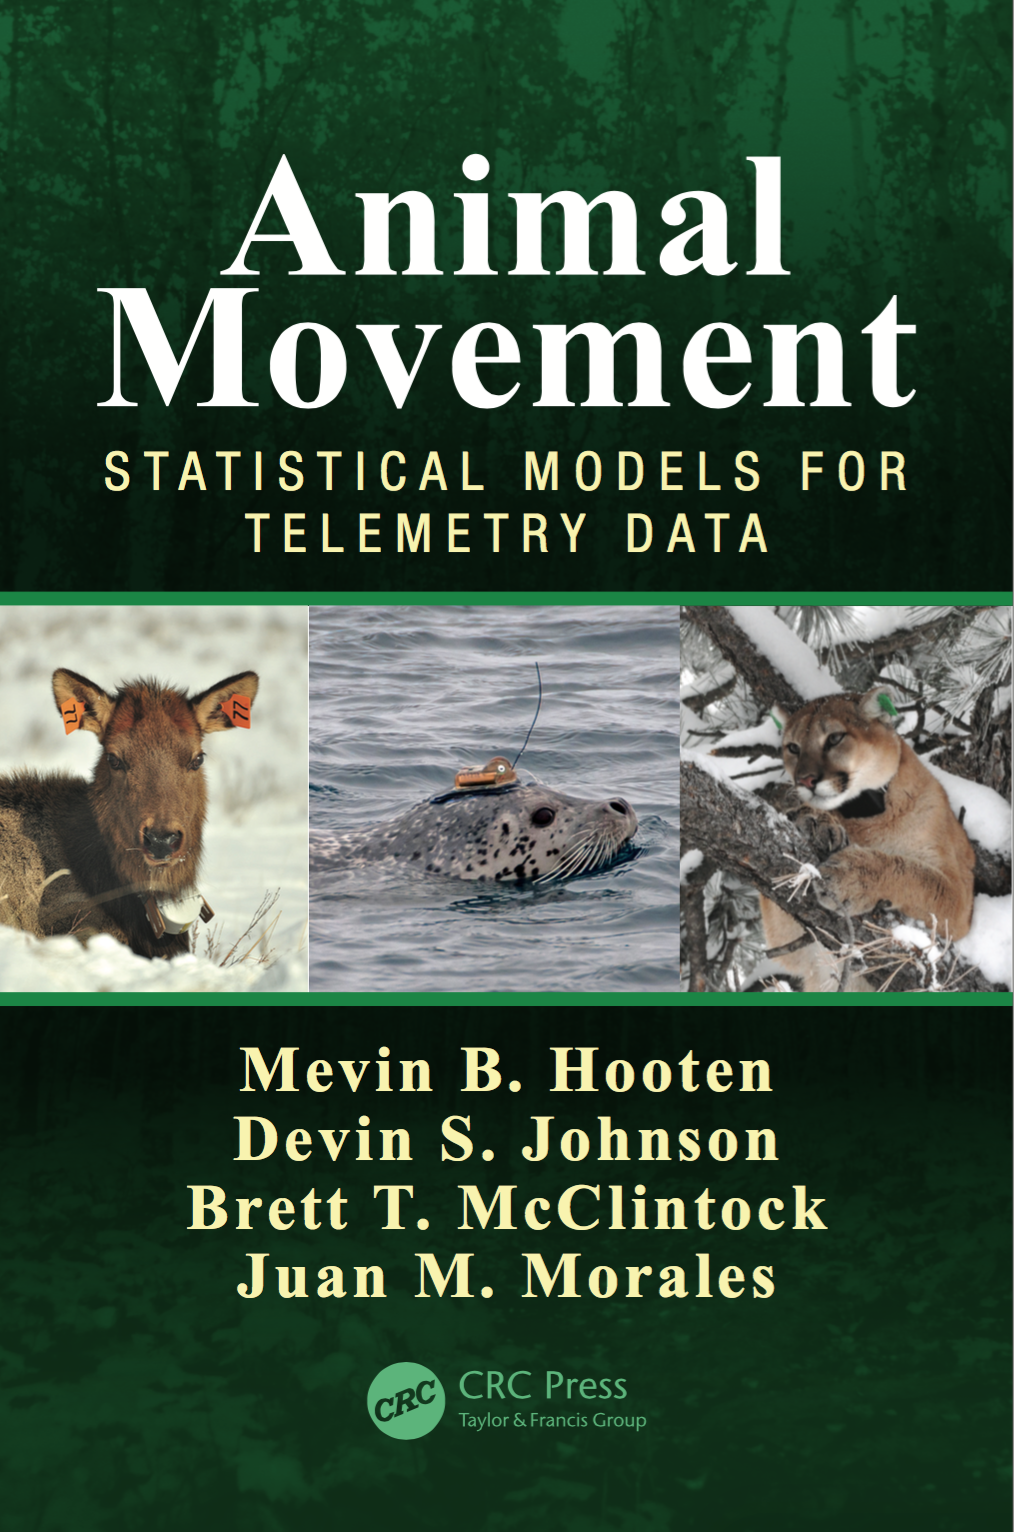
\includegraphics[height=0.75\textheight]{Book_Cover_Final.png}
\end{center}

\column{0.6\textwidth}
\begin{itemize}
	\item Available from Amazon (\$86)
	\item Soon to be available at the MML library
	\item Borrow from me (maybe Brett)
\end{itemize}

\end{columns}
\end{frame}


%%%%%%%%%%%%%%%%%%%%%%%

{
\setbeamercolor{background canvas}{bg=dark-gray}
\renewcommand{\baselinestretch}{2}\normalsize

\begin{frame}
\nt{\Huge Part I}
\bigskip

\nt{\Huge Mathematics of animal movement}
\end{frame}
}


%%%%%%%%%%%%%%%%%%%%%%%%%

{
\setbeamercolor{background canvas}{bg=dark-gray}
\begin{frame}
\textcolor{noaaturq}{\Huge Discrete-time models}
\end{frame}
}

%%%%%%%%%%%%%%%%%%%%%%%%%

\begin{frame}
\ft{Time series models}
Telemetry data are thought of as predominately {\it spatial}
\begin{itemize} 
	\item We display them on 2d maps
	\item We want to know something about {\it space} use
	\item We want to know which spatial locations are selected over others
\end{itemize}
  
Most mathematical models and statistical analysis view telemetry data as {\it time series} processes where a realization occurs in geographical space \medskip

{\Large \textcolor{noaaturq}{Notation (discrete time)}}
\begin{itemize}
\item $\bmu_t = (\mu_{x,t}, \mu_{y,t})$ is the location of the animal at time $t$.
\item $\bs_t = (s_{x,t}, s_{y,t})$ is the observed location at time $t$.
\item $d\bmu_t = \bmu_t - \bmu_{t-1}$ is {\em movement}!
\end{itemize}

\end{frame}

%%%%%%%%%%%%%%%%%%%%%%%%

\begin{frame}
\ft{Random walk}
$$\bmu_t = \bmu_{t-1} + \be_t$$
 
$$[\be_t] = N(0,\boldsymbol{\Sigma})$$

\begin{itemize}
\item The movements, $d\bmu_t = \be_t$ are all independent of each other.
\item Typically $\boldsymbol{\Sigma} \equiv \sigma^2\mathbf{I}$, so, $\mu_{x,t}$ is independent of $\mu_{y,t}$
\end{itemize}
\medskip

\textcolor{noaaturq}{\Large An unconditional view}

We can rewite the RW using the accumulation of movements:
$$
\begin{aligned}
\bmu_t &= \bmu_{t-1} + \be_t \\ 
&= \bmu_{t-2} + \be_{t-1} + \be_t \\ 
&=\bmu_0 + \sum_{i=1}^t \be_i
\end{aligned}
$$

\end{frame}

%%%%%%%%%%%%%%%%%%%%%%%%%%%%%%%%%%%%

\begin{frame}
rw demo
\end{frame}

%%%%%%%%%%%%%%%%%%%%%%%%%

\begin{frame}
\ft{Vector autoregressive models (VAR)}

Let's suppose that an animal would like to stay close to some focal point, say $\bar\bmu$. 
\bigskip

\textcolor{noaaturq}{\Large VAR(1) model}

$$
\begin{aligned} \bmu_t &= \bar\bmu + \mathbf{M}(\bmu_{t-1}-\bar\bmu) + \epsilon_t \\ 
&= (\mathbf{I}-\mathbf{M})\bar\bmu + \mathbf{M}\bmu_{t-1} + \epsilon_t 
\end{aligned}
$$

\begin{itemize}
\item Weighted mean of last location and point of attraction
\item If $\mathbf{M} \equiv \rho\mathbf{I}$ and $|\rho|<1$ then as $t \to \infty$ $$[\bmu_t] = N\left(\bar\bmu, \frac{1}{1-\rho^2}\boldsymbol{\Sigma}\right)$$
\item What happens if $\rho \to 1$?
\end{itemize}

\end{frame}


%%%%%%%%%%%%%%%%%%%%%%%%%%%%%%

\begin{frame}
var(1) demo
\end{frame}

%%%%%%%%%%%%%%%%%%%%%%%%%

\begin{frame}
\ft{Modeling velocity}

\begin{itemize}
\item Rule 1. velocity $\ne$ speed!
\item We are thinking of velocity in the physics sense. Speed is the magnitude of velocity. 
$$\mbox{velocity = derivative of location process}$$
\end{itemize}
\bigskip

What does that mean for our random walk models in discrete-time? 

$$
\begin{aligned}
\mbox{velocity} &= d\bmu_t \\ 
&= \bmu_t-\bmu_{t-1} 
\end{aligned}
$$
\end{frame}

%%%%%%%%%%%%%%%%%%%%%%%%%%%

\begin{frame}
\ft{VAR(1) model for velocity}

Instead of directly modeling location as a VAR(1), we can model movement (velocity) with a VAR(1)

$$d\bmu_t = \mathbf{M}d\bmu_{t-1} + \be_t$$
Now, the movement steps are {\em correlated} compared to a simple random walk. 
\medskip

We might call this model  a {\em correlated random walk}
\medskip

\textcolor{noaaturq}{\Large Why CRW?}
\begin{itemize}
\item Step at time $t$, $d\bmu_t$, tends to be similar to the previous step, $d\bmu_{t-1}$
\item The correlation in steps produces a {\em superdiffusive} process for $\mu_t$
\item Why is it useful? Better model of movement in the short term (i.e., $t<<\infty$)
\end{itemize}
\end{frame}

%%%%%%%%%%%%%%%%%%%%%%%%%

\begin{frame}
\ft{Correlated random walk}

If we model $d\bmu_t = \mathbf{M}\ d\bmu_{t-1} + \be_t$, what does this mean for  $\bmu_t$?

Recall we can always write the position process like this:
$$
\begin{aligned}
\bmu_t &= \bmu_{t-1} + (\bmu_t-\bmu_{t-1}) \\ 
&= \bmu_{t-2} + (\bmu_{t-1}-\bmu_{t-2}) + (\bmu_t-\bmu_{t-1}) \\ 
&\vdots \\ 
&= \bmu_0 + \sum_{i=1}^t (\bmu_{i}-\bmu_{i-1}) \\ 
&= \bmu_0 + \sum_{i=1}^t d\bmu_i 
\end{aligned}
$$
Notice that there was no distributional assumption for $d\bmu_t$. 

It's a simple recursion. 

\end{frame}

%%%%%%%%%%%%%%%%%%%%%%%%%

\begin{frame}
\ft{Correlated random walk}

The CRW can also be represented as a VAR(2) process

$$
\begin{aligned}
\bmu_t &= \bmu_{t-1} + \mathbf{M}d\bmu_{t-1} + \be_t \\ 
&= \bmu_{t-1} + \mathbf{M}(\bmu_{t-1}-\bmu_{t-2}) + \be_t \\ 
&= (\mathbf{I}+\mathbf{M})\bmu_{t-1} - \mathbf{M}\bmu_{t-2} + \be_t
\end{aligned}
$$
Current location is a weighted sum of previous {\em two} locations
\medskip

\textcolor{noaaturq}{\large The $\mathbf{M}$ matrix}

Turning angle specification

$$
\mathbf{M} = \gamma\left[\begin{array}{cc} \cos(\theta) & -\sin(\theta) \\ \sin(\theta) & \cos(\theta) \end{array} \right]
$$
\begin{itemize}
\item $\theta$ represents mean turning angle (probably close to 0) 
\item $0 < \gamma < 1$  controls the correlation in velocity
\end{itemize}

\end{frame}


%%%%%%%%%%%%%%%%%%%%%%%%

\begin{frame}
\ft{Correlated random walk}
Let's suppose $\theta$ = 0, so,
$$\mathbf{M} = \gamma \mathbf{I}$$
\medskip

Then $\mbox{corr}(d\bmu_t, d\bmu_s) = \gamma^{|t-s|}$
\bigskip

But let's reparameterize $\gamma = e^{-\beta}$, then 
\begin{itemize}
\item $\gamma \approx 1 \implies \beta \approx 0$ 
\item $\gamma \approx 0 \implies \beta \mbox{ very large (sort of)}$ 
\end{itemize}

So, $\mbox{corr}(d\bmu_t, d\bmu_s) = e^{-\beta|t-s|}$

\end{frame}

%%%%%%%%%%%%%%%%%%%%%%%
{
\setbeamercolor{background canvas}{bg=dark-gray}
\begin{frame}
\textcolor{noaaturq}{\Huge Continuous-time models}
\end{frame}
}

%%%%%%%%%%%%%%%%%%%%%%%%

\begin{frame}
\ft{Brownian motion}
Forms the basis of all continuous-time models\medskip

Random walk in continuous-time \medskip

So, let's start from the beginning...
$$
\begin{aligned}
\bb_t &= \bb_{t-1} + \be_t \\
&= \bb_0 + \sum_{j=1}^{t}\left[\bb_j-\bb_{j-1}\right] \\
&= \bb_0 + \sum_{j=1}^{t} d\bb_j
\end{aligned}
$$
Recall,

$[d\bb_j] = N(\mathbf{0},\sigma^2\mathbf{I})$ and $d\bb_j$ is indep. of $d\bb_i$

(usually, $\bb_0 = \mathbf{0}$ and $\sigma=1$)

\end{frame}

%%%%%%%%%%%%%%%%%%%%%%%

\begin{frame}
\ft{Brownian motion}
We can get to continuous-time by making the time gaps, $\delta = \tau_j-\tau_{j-1}$, smaller and smaller

\begin{block}{Definition}
$$
\begin{aligned}
\bb_\tau &= \lim_{\delta \to 0} \sum_{j=1}^\tau d\bb_j \\
&= \int_0^\tau d\bb_u
\end{aligned}
$$
\end{block}

\begin{itemize}
\item $d\bb_\tau$ is infinitely rough
\item $\bb_\tau$ is a continuous function of time with no classical derivative 
\item Trivia fact for the bar: Here `$\int$' represents an Ito integral

\end{itemize}

\end{frame}

%%%%%%%%%%%%%%%%%%%%%%%

\begin{frame}
BM example
\end{frame}

%%%%%%%%%%%%%%%%%%%%%%%%

\begin{frame}
\ft{Brownian motion}
\begin{block}{Properties}
\begin{itemize}
\bigsp
\item $\mbox{Mean}[\bb_\tau] = \mathbf{0}$
\item $\mbox{Var}[\bb_\tau] =  \tau \mathbf{I}$
\item Independent increments ...\\
\medskip
$\bb_{\tau_2}-\bb_{\tau_1}$ is independent of $\bb_{\tau_4}-\bb_{\tau_3}$ if $[\tau_1, \tau_2]$ does not overlap $[\tau_3,\tau_4]$.
\end{itemize}
\end{block}
\end{frame}

\begin{frame}
\ft{Ornstein-Uhlenbeck process}

What about an AR(1) version of BM?

$$
\begin{aligned}
(1)\quad \bmu_t &= \gamma(\bmu_{t-1}-\bar\bmu) + \be_t \\ \pause
&\\
(2)\quad \bmu_t &= \bmu_0 + \sum_{j=1}^t [\bmu_j-\bmu_{j-1}] \\ 
&= \bmu_0 + \sum_{j=1}^t (\gamma-1)(\bmu_{j-1})-\bar\bmu) + \sum_{j=1}^t \be_j \\ \pause
(3)\quad \bmu_\tau &= \bmu_0 + \int_0^\tau (\gamma-1)(\bmu_u-\bar\bmu)du + \sigma \bb_u \pause
\end{aligned}
$$ 
which implies ($\beta=1-\gamma$)
$$
d\bmu_\tau = -\beta(\bmu_\tau-\bar\bmu)d\tau + \sigma d\bb_\tau
$$

\end{frame}

%%%%%%%%%%%%%%%%%%%%%%%

\begin{frame}
\ft{Stochastic differential equations}
General form
$$
d\bmu_\tau = g(\bmu_\tau)dt + h(\bmu_\tau)d\bb_\tau
$$

Solution (assume $h\equiv\sigma$)
$$
\bmu_\tau = \bmu_0 + \int_0^\tau g(\bmu_u)du + \sigma\bb_\tau
$$

For OU model
$$
\bmu_\tau = e^{-\beta t}\bmu_0 + (1-e^{-\beta \tau})\bar\bmu + \boldsymbol{\zeta}_\tau
$$
where $[\boldsymbol{\zeta}_\tau] = N\left(\mathbf{0}, \frac{\sigma^2(1-e^{-2\beta \tau})}{2\beta}\mathbf{I}\right)$

\end{frame}

%%%%%%%%%%%%%%%%%%%%%%%

\begin{frame}
\ft{Integrated SDEs (Velocity modeling)}
New notation:
\begin{itemize}
\item $\bv_\tau$ = velocity at time $\tau$
\item $H(\bmu_\tau)$ = potential function to control movement
\item $\nabla H(\cdot)$ = spatial gradient of $H$
\end{itemize}

\begin{block}{Movement ISDE}
$$
\begin{aligned}
&d\bv_\tau = -\beta\{\bv_\tau -\nabla H(\bmu_\tau) \} + \sigma d\bb_\tau \\
&d\bmu_\tau = \bv_\tau \\
&\Downarrow \\
&\bmu_\tau = \int_0^\tau \bv_u du
\end{aligned}
$$
\end{block}

\end{frame}

%%%%%%%%%%%%%%%%%%%%%%%

\begin{frame}
\ft{Continuous-time CRWs}
\begin{block}{CTCRW}
$$
\begin{aligned}
&d\bv_\tau = -\beta \bv_\tau + \sigma d\bb_\tau \\
&d\bmu_\tau = \bv_\tau \\
&\Downarrow \\
&\bv_\tau = \mbox{OU}(\beta, \sigma)\\
&\bmu_\tau = \bmu_0 + \int_0^\tau \bv_u du
\end{aligned}
$$
\end{block}
\begin{itemize}
\item $\bv_\tau$ is an Ornstein-Uhlenbeck (continuous-time AR(1)) process
\item $H\equiv 0$
\item $\bmu_\tau$ accumulates instantaneous changes in location
\end{itemize} 

\end{frame}

%%%%%%%%%%%%%%%%%%%%%%%%%

\begin{frame}
\ft{Continuous-time CRWs}
Some useful properties: 
\medskip

\begin{itemize}
\bigsp
\item $\bv_{\tau+\delta} = \bv_\tau e^{-\beta\delta} + \boldsymbol{\zeta}_{\tau+\delta}$, 
\item $\bmu_{\tau+\delta} = \bmu_\tau + \bv_\tau\left(\frac{1-e^{-\beta\delta}}{\beta}\right) + \boldsymbol{\xi}_{\tau+\delta}$
\item $\be_{\tau+\delta} = (\boldsymbol{\zeta}_{\tau+\delta}, \boldsymbol{\xi}_{\tau+\delta})$ are zero mean independent (through time) normal errors that depend only on $\delta$, $\beta$, and $\sigma$ ({\bf Not} $\tau$!) 
\item Can we write $\bmu_{\tau+\delta}$ just as a function of $\bmu_\tau$? \medskip \\
{\bf No}. Distribution of $\bmu_\tau$ is a function of the whole $\bmu_u$, $u<\tau$.
\end{itemize}
\vfill
\end{frame}


%%%%%%%%%%%%%%%%%%%%%%%
\begin{frame}
\ft{Continuous-time CRWs}
Some more properties: 
\medskip

\begin{itemize}
\bigsp
\item $\mbox{corr}[\bv_{\tau+\delta},\bv_\tau] = e^{-\beta\delta}$,\\
$\approx 0$ for $\beta$ large\\
$\approx 1$ for $\beta$ small
\item $\bmu_\tau \to$ Brownian motion as $\beta$ becomes large\\
$\bmu_\tau$ becomes very smooth as $\beta$ becomes small
\item $\bv_{\tau+\delta}$ roughly indep. of $\bv_\tau$ at time gap $\delta = 3/\beta$, so, ...\medskip \\
$\bmu_\tau,\ \bmu_{\tau+3/\beta},\ \bmu_{\tau+6/\beta},\dots$ not really distinguishable from Brownian motion
\end{itemize}
\vfill
\end{frame}


%%%%%%%%%%%%%%%%%%%%%%%
\begin{frame}
\ft{Continuous-time CRWs}
What about $H(x,y) \ne 0$? The future?
\medskip

\begin{block}{Numerical solution to general ISDE model}
for small $\delta$

$\bv_{\tau+\delta} \approx -\beta(\bv_\tau - \nabla H(\bmu_\tau) )\delta + \be_{\tau+\delta};\qquad [\be_{\tau}]=N(\mathbf{0},\sigma^2\delta\mathbf{I})$
\medskip

$\bmu_{\tau+\delta} \approx \bmu_\tau + \bv_\tau \delta \implies \bv_\tau \approx (\bmu_{\tau+\delta}-\bmu_\tau)/\delta$
\bigskip

Resulting approximation:

$
\bmu_{\tau+2\delta} = (2-\beta\delta)\bmu_{\tau+\delta} -  (1-\beta\delta)\bmu_\tau + \beta\delta^2 \nabla H(\bmu_\tau) + \be_{\tau+\delta}
$
\end{block}
\medskip

Notice that $\bv_\tau$ process disappears and there is a spatial component, $\nabla H(\bmu_\tau)$! Something missing from the standard CTCRW model.


\end{frame}


%%%%%%%%%%%%%%%%%%%%%%%


{
\setbeamercolor{background canvas}{bg=dark-gray}
\renewcommand{\baselinestretch}{2}\normalsize

\begin{frame}
\nt{\Huge Part II}
\bigskip

\nt{\Huge Statistics of animal movement}
\end{frame}
}

%%%%%%%%%%%%%%%%%%%%%%%%

{
\setbeamercolor{background canvas}{bg=dark-gray}
\begin{frame}
\textcolor{noaaturq}{\Huge Inference refresher}
\end{frame}
}

%%%%%%%%%%%%%%%%%%%%%%%%

\begin{frame}
\ft{Maximum likelihood estimation}
\begin{block}{Notation}
\begin{itemize}
\item $\bd = (d_1,\dots, d_n)$ = vector general data
\item $\bt$ general set a parameters
\item $[d_i|\bt]$ = probability model that generates data
\item $L(\bt|\bd)$ = likelihood function \\
typically $L(\bt|\bd) = [\bd|\bt] = \prod_i[d_i|\bt]$
\end{itemize}
\end{block}
\bigskip

MLE is very straightforward (in theory) ...

$$\hat\bt = \mbox{max}_{\bt} \{\log L(\bt|\bd)\}$$ \pause

boom!

\end{frame}

%%%%%%%%%%%%%%%%%%%%%%%%

\begin{frame}
\ft{MLE details}

\nt{Large sample theory}
\medskip

If $\bd = (d_1 \dots d_n)$ is `large' then 
$$\hat\bt \sim N(\bt, -\mathbf{H}_{\bt}^{-1}),$$
where $\mathbf{H}_{\bt}$ is the Hessian matrix of $\log L(\bt|\bd)$.
\bigskip

\pause

\nt{Dependent data}
\medskip

If the data are dependent, then $[\bd|\bt] \ne \prod_i [d_i|\bt]$. 
\medskip

$[\bd|\bt] = [d_1|\bt]\times [d_2|d_1,\bt]\times [d_3|d_1,d_2,\bt] \times \dots \times [d_n|d_1,\dots,d_{n-1},\bt]$
\medskip

If we're lucky, our data are Markov
\medskip

$[\bd|\bt] = [d_1|\bt]\times [d_2|d_1,\bt]\times [d_3|d_2,\bt] \times \dots \times [d_n|d_{n-1},\bt]$

\vfill

\end{frame}

%%%%%%%%%%%%%%%%%%%%%%%%

\begin{frame}
\ft{MLE details}

\nt{Missing `data' likelihoods}
\medskip 

$L(\bt|\bd_{obs}) = [\bd_{obs}|\bt] = \int [\bd_{obs}|\bd_{mis},\bt]\ [\bd_{mis}|\bt] d\bd_{mis}$
\bigskip

\nt{Penalized likelihood}
\medskip

Sometimes the likelihood is hard to maximize or parameters are not full identifiable. So, a penalty term is added
\medskip

$\log L_p(\bt|\bd) = \log L(\bt|\bd) + \kappa J(\bt)$
\medskip

We'll see some examples laster. But this is how spline regressions are fit (e.g., see {\tt mgcv} package).

\vfill
\end{frame}

%%%%%%%%%%%%%%%%%%%%%%%%%%

\begin{frame}
\ft{Bayesian inference}

Instead of a fixed quantity, $\bt$, is treated like a random variable itself. Before any data is collected, we might model our uncertainty about the value of $\bt$ with the probability distribution $[\bt]$. This is the `prior' distribution.
\medskip

We already have the data model $[\bd|\bt] = L(\bt|\bd)$
\medskip

\begin{block}{Bayes rule and posterior distribution}

$$[\bt|\bd] = \frac{L(\bt|\bd)\ [\bt]}{\int [\bd|\bt']\ [\bt'] d\bt'}$$
Or, we can look at it on the log scale
$$\log [\bt|\bd] = \log L(\bt|\bd) + \log [\bt] - const.$$
\end{block}

\end{frame}

%%%%%%%%%%%%%%%%%%%%%%%%

\begin{frame}
\ft{Bayes inference details}
\nt{How do we work with a posterior distribution?}
\begin{itemize}
\item $\hat\theta$ = mean, median or mode
\item $SE$ of $\hat\bt$ = SD of $[\bt|\bd]$
\item Interval estimates = $(\hat\bt_l,\hat\bt_u)$ such that $Pr(\hat\bt_l < \bt|\bd < \hat\bt_u) = 0.95$. These are called `credible intervals'
\end{itemize}

\vfill

\nt{How do we find these for general posteriors?}
\begin{itemize}
\item Approximate with a sample $\bt_1,\dots,\bt_m$ from $[\bt|\bd]$ and use sample versions
\item Numerically (including Monte Carlo) approximate integrals necessary
\item Approximate with known distribution that is similar
\end{itemize}

\end{frame}
%%%%%%%%%%%%%%%%%%%%%%%%%



{
\setbeamercolor{background canvas}{bg=dark-gray}
\begin{frame}
\textcolor{noaaturq}{\Huge Telemetry analysis}
\end{frame}
}

%%%%%%%%%%%%%%%%%%%%%%%%

\begin{frame}
\ft{State-space models}

\nt{Notation}
\begin{itemize}
\item $\bs_1,\dots,\bs_n$ are observed locations
\item $\tau_1,\dots,\tau_n$ are the observation times
\item $\bmu_\tau$ is the continuous path of the animal at time $\tau$
\item $\bv_\tau$ is the velocity at time $\tau$
\item $\ba_\tau = (\mu_{\tau,x}, \nu_{\tau,x}, \mu_{\tau,y}, \nu_{\tau,y})$,
\end{itemize}

\end{frame}

%%%%%%%%%%%%%%%%%%%%%%%%%%%

\begin{frame}
\ft{State-space models}

\begin{block}{CTCRW model}
$$
\begin{aligned}
\bs_i &= \mathbf{z}'\ba_{\tau_i} + \be_i\\
\ba_{\tau_{i+1}} &= \mathbf{T}_i \ba_{\tau_i} + \boldsymbol{\eta}_i
\end{aligned}
$$
\begin{itemize}
\item $[\be_i] = N(\mathbf{0}, \mathbf{V}_i)$; $\mathbf{V}_i$ is the location error variance.
\item $\mathbf{z} = (1,0,1,0)$
\item $\mathbf{T}_i$ is a function of $\beta$ and $\delta_i = \tau_{i+1}-\tau_i$
\item $[\boldsymbol{\eta}_i] = N(\mathbf{0}, \mathbf{Q}_i)$
\item $\mathbf{Q}_i$ depends only on $\beta$, $\delta_i$, and $\sigma$
\end{itemize}

\end{block}

\end{frame}

%%%%%%%%%%%%%%%%%%%%%%%%%%

\begin{frame}
\ft{Temporally dynamic CTCRW}

The parameters do not have to remain constant over time!
\begin{itemize}
\item $\tau_1^*,\dots, \tau_m^*$ are known times where $\beta$ and $\sigma$ {\em can} change
\item Define model as before based on merged observation and changepoint times, $\tau_1,\dots,\tau_{n+m}$
\end{itemize}

\begin{block}{Temporally dynamic movement model}
$$
\begin{aligned}
&\bs_i = \left\{\begin{array}{ll} \mathbf{z}'\ba_{\tau_i} + \be_i & \mbox{for } \tau_i \mbox{ an observed time} \\
\mbox{NA } & \mbox{for } \tau_i \mbox{ in } \tau_1^*,\dots,\tau_m^* \end{array} \right. \\
&\ba_{\tau_{i+1}} = \mathbf{T}_i \ba_{\tau_i} + \boldsymbol{\eta}_i
\end{aligned}
$$
\end{block}

Movement model is still continuous in time! 

\end{frame}

%%%%%%%%%%%%%%%%%%%%%%%%

\begin{frame}
\ft{Kalman filter}
Method to calculate likelihood, {\em NOT} a model!
\medskip

\begin{block}{Likelihood for state-space models}
$$
\begin{aligned}
&L(\bt|\bs_{1:n}) = \prod_i[\bs_{i+1}|\bs_{1:i},\bt] \\
&= \int [\bs_1|\ba_{\tau_1},\theta]\ [\ba_{\tau_1}|\bt]\dots [\ba_{\tau_i}|\ba_{\tau_{i-1}},\bt] \times \dots\\
&\qquad\qquad \times [\bs_{n}|\ba_{\tau_{n+m}},\theta]\ [\ba_{\tau_{n+m}}|\ba_{\tau_{n+m-1}},\bt] d\ba_{1:n+m}
\end{aligned}
$$
\end{block}
\medskip

\nt{Kalman filter} is a numerical algorithm that allows calculation of $L(\bt|\bs_1,\dots,\bs_n)$ in an efficient manner. 
\begin{itemize}
\item moves forward through the complete likelihood integrating on the way
\item requires linear form and normal errors 
\end{itemize} 

\end{frame}

%%%%%%%%%%%%%%%%%%%%%%%%%
\begin{frame}
\ft{Kalman smoother}

Obtain predictions from model fit
\begin{itemize}
\item optimal predictor $\hat\ba_i = E[\ba_i|\bs_{1:n},\bt]$
\item prediction errors $\widehat{\mbox{var}}(\hat\ba_i) = Var[\ba_i|\bs_{1:n},\bt]$
\end{itemize}
\bigskip\bigskip

\nt{Kalman smoother} is an algorithm to calculate mean and variance of $[\ba_i|\bs_{1:n}, \bt]$
\begin{itemize}
\item uses output from Kalman filter to go backwards through the model/data to calculate these quantities
\item $\ba_i|\bs_{1:n},\bt$ is normally distributed. 
\end{itemize}


\end{frame}

%%%%%%%%%%%%%%%%%%%%%%%%

\begin{frame}
\ft{Practical Bayesian inference}

\nt{Posterior }

$$
\begin{aligned}[]
[\bt,\ba|\bs] &\propto [\bs|\ba,\bt]\ [\ba|\bt]\ [\bt] \\
%&= [\ba|\bs,\bt]\ [\bs|\bt]\ [\bt] \\
&\propto [\ba|\bs,\bt]\ [\bt|\bs]
\end{aligned}
$$

\nt{Approach}
\begin{enumerate}
\bigsp
\item Approximate $[\bt|\bs]$ with something easy to sample from, say $[\bt|\bs]^*$
\item Draw $\bt^{(i)} \sim [\bt|\bs]^*$ then draw $\ba^{(i)} \sim [\ba|\bt^{(i)}, \bs]$\\
($[\ba|\bt^{(i)}, \bs]$ easy to sample from using KFS algorithms)
\item $(\bt^{(1)},\ba^{(1)}),\dots,(\bt^{(K)},\ba^{(K)})$ is a posterior sample
\item $m_i = f(\bt^{(i)},\ba^{(i)})$ will be a sample from $[m|\bs]$
\end{enumerate}

\end{frame}

%%%%%%%%%%%%%%%%%%%%%%%%

\begin{frame}
\ft{Approximating $[\bt|\bs]$}
\begin{itemize}
\bigsp
\item Normal approximation
	\begin{enumerate}
	\item maximize $\log[\bs|\bt] + \log[\bt] = L_p(\bt|\bs)$ (penalized likelihood)
	\item $[\bt|\bs]^* = N\left(\hat\bt, -\mathbf{H}_{\hat\bt}^{-1}\right)$ (possibly truncated)
	\end{enumerate}
\item Importance sampling (exact sample)
	\begin{enumerate}
	\item sample $\tilde\bt^{(k)}\sim q(\bt)$ (maybe normal from last item)
	\item form weights $w_k = [\tilde\bt^{(k)}|\bs]/q(\tilde\bt^{(k)})$
	\item sample $\bt^{(i)}$ from $\tilde\bt^{(1)},\dots,\tilde\bt^{(K)}$ with prob. $\propto w_1,\dots,w_K$
	\end{enumerate}
\item Deterministic sample (INLA)
	\begin{enumerate}
	\item sample $\tilde\bt^{(k)}$ from deterministic grid
	\item form weights $w_k = [\tilde\bt^{(k)}|\bs]$
	\item sample $\bt^{(i)}$ from $\tilde\bt^{(1)},\dots,\tilde\bt^{(K)}$ with prob. $\propto w_1,\dots,w_K$
	\end{enumerate}

\end{itemize}

\end{frame}

%%%%%%%%%%%%%%%%%%%%%%%%%

\begin{frame}
\ft{Process imputation}

Allows us to account for location uncertainty in other analysis of movement data

Assume we know $\bmu_\tau$ on a sufficiently fine time scale 

Analysis desired $\mathbf{y} = \mathbf{f}(\bmu)$




\end{frame}

%%%%%%%%%%%%%%%%%%%%%%%%

\begin{frame}
\ft{Process imputation}

\end{frame}

%%%%%%%%%%%%%%%%%%%%%%%%
{
\usebackgroundtemplate{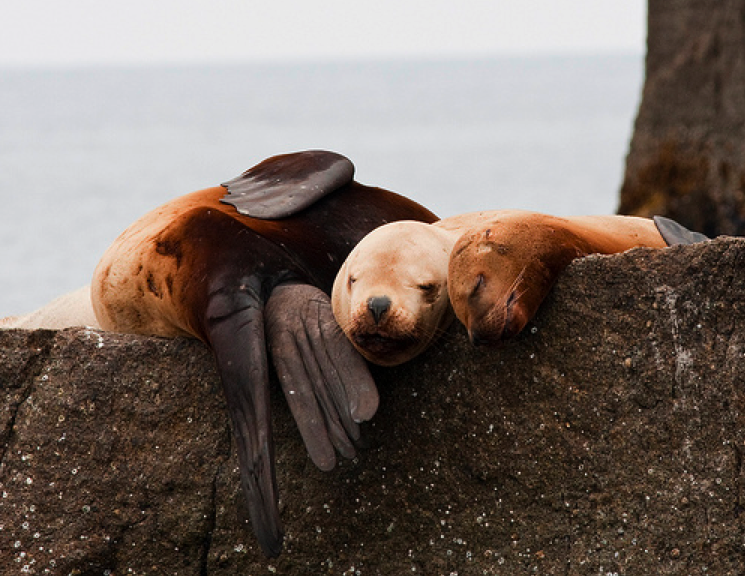
\includegraphics[width=\paperwidth]{ssl_sleep.png}}
\setbeamercolor{frametitle}{fg=noaaturq}
\begin{frame}[t]
\frametitle{That's all the math folks!}
Anyone awake?
\vspace*{\fill}
%\begin{center}
%\includegraphics[width=\textwidth]{nfs_pup_questions.png}
%\end{center}
\end{frame}
}





\end{document}
